\section{System Design}
The core idea of the Mobility Feature Package is to provide a very simple programming interface such that computing features can be done with very few lines of code. This requires hiding the implementation of the package such that the programmer has very limited ways in which he/she can interface with it. The design of the package API went through two main iterations which consisted of many smaller iterations. Mainly, the difference between the final iteration and the earlier iterations is the amount of code required by the programmer to compute features. Early iterations put the responsibility on the application programmer to manage historical data. After developing the field study app discussed in chapter \ref{chapter:06} it was decided to move most of this logic inside the package. The final iteration is the one discussed in this thesis including the choices and lessons learned on the way of designing and developing it.\\

The flowchart in Figure \ref{fig:flowchart-features} displays the task which the software system must be able to carry out, as well as which parts are done by the package, and which are done by the programmer. Namely, the task of collecting location data was chosen to be carried out by the programmer which was a major design choice. Two reasons led to this decision, the first of which being that the Mobility Features Package becomes more loosely coupled. Secondly, it gives the programmer flexibility to collect location data in the way they see fit. Thirdly, if the package was to implement location data collection then it becomes harder to maintain since any change to the location plugin would imply changes to the Mobility Features Package as well. 

\begin{figure}[h]
    \centering
    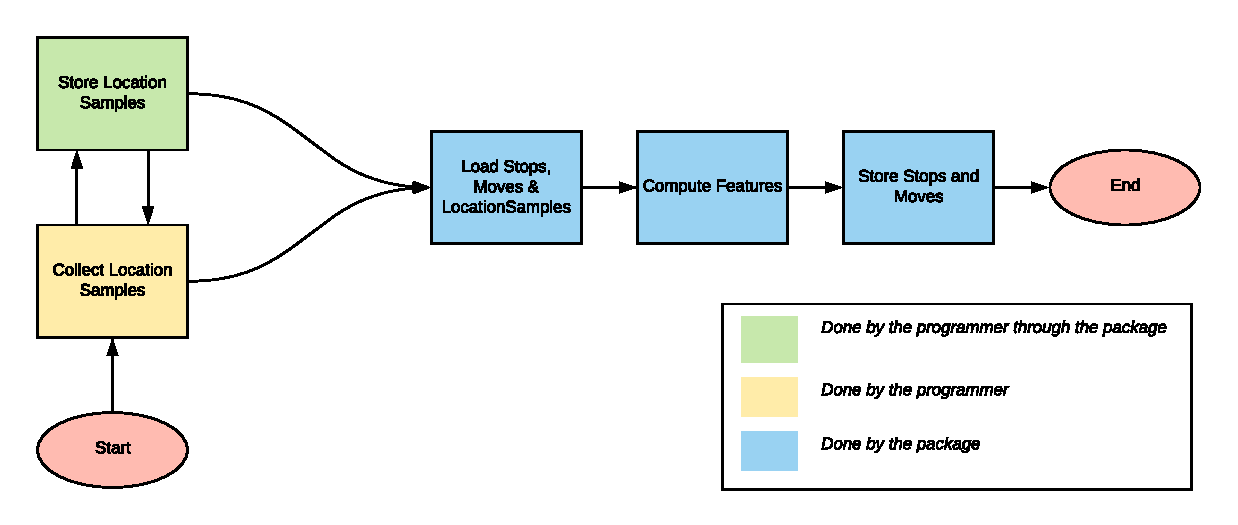
\includegraphics[width=\textwidth]{images/diagrams/flowchart.pdf}
    \caption{Flowchart of the feature computation process}
    \label{fig:flowchart-features}
\end{figure}


\subsection{Component Overview}
Figure \ref{fig:component-diagram-internal} displays how the final iteration looks like as a software system: The main component is the Context Generator component which is the interface that the programmer will have access to. This component exposes two interfaces to the programmer allowing the user to store their collected LocationSamples as well as generate a \textit{Mobility Context}, which is an abstraction containing all the daily features. The two exposed interfaces are provided by the programmer through the mobile application. The Context Generator is also responsible for storing and loading data via the Mobility Serializer component, here the \textit{Serializable} type refers to any data type that needs to be stored as historical data.

\begin{figure}[h]
\centering
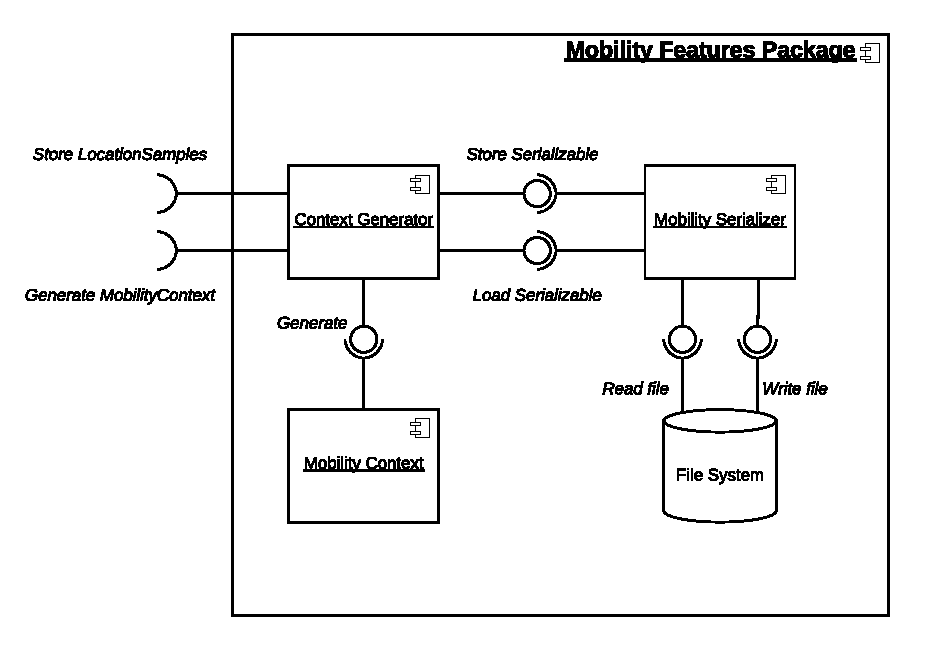
\includegraphics[width=0.8\textwidth]{images/diagrams/component-internal.pdf}
\caption{Component diagram for the Mobility Feature Package from an internal point of view}
\label{fig:component-diagram-internal}
\end{figure}

Figure \ref{fig:component-diagram-external} shows the external software system that includes the mobile application using the package. The design choice of letting the programmer collect location data themselves is also reflected in the usage of an external location plugin. This location plugin will deliver location Data Transfer Objects (DTOs) as defined by y Fowler \cite{fowler-PEEA} [p. 401] to the mobile health application. These objects hold location data, i.e. latitude, longitude, and a timestamp and can be converted to LocationSamples and saved through the \textit{}


\begin{figure}[h]
\centering
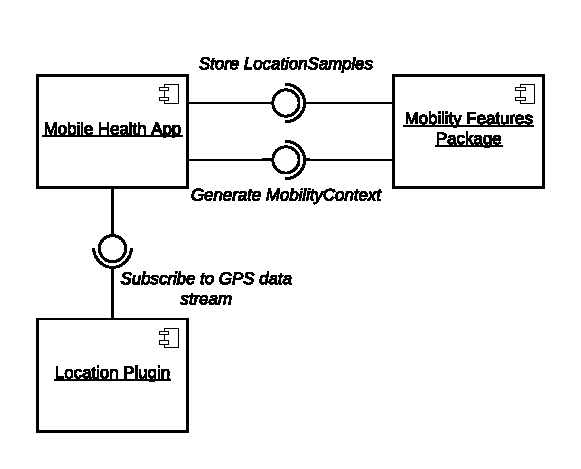
\includegraphics[width=0.7\textwidth]{images/diagrams/component-external.pdf}
\caption{Component diagram for the Mobility Feature Package from an internal point of view}
\label{fig:component-diagram-external}
\end{figure}


\subsection{Sequence Overview}
To display the information flow between the components, sequence diagrams are used. Figure \ref{fig:sequence-diagram-external} shows the system from an external point of view, where the application subscribes to location updates via the location plugin, saves location data via the Mobility Features Package and generates a Mobility Context through it. 

\begin{figure}[h]
\centering
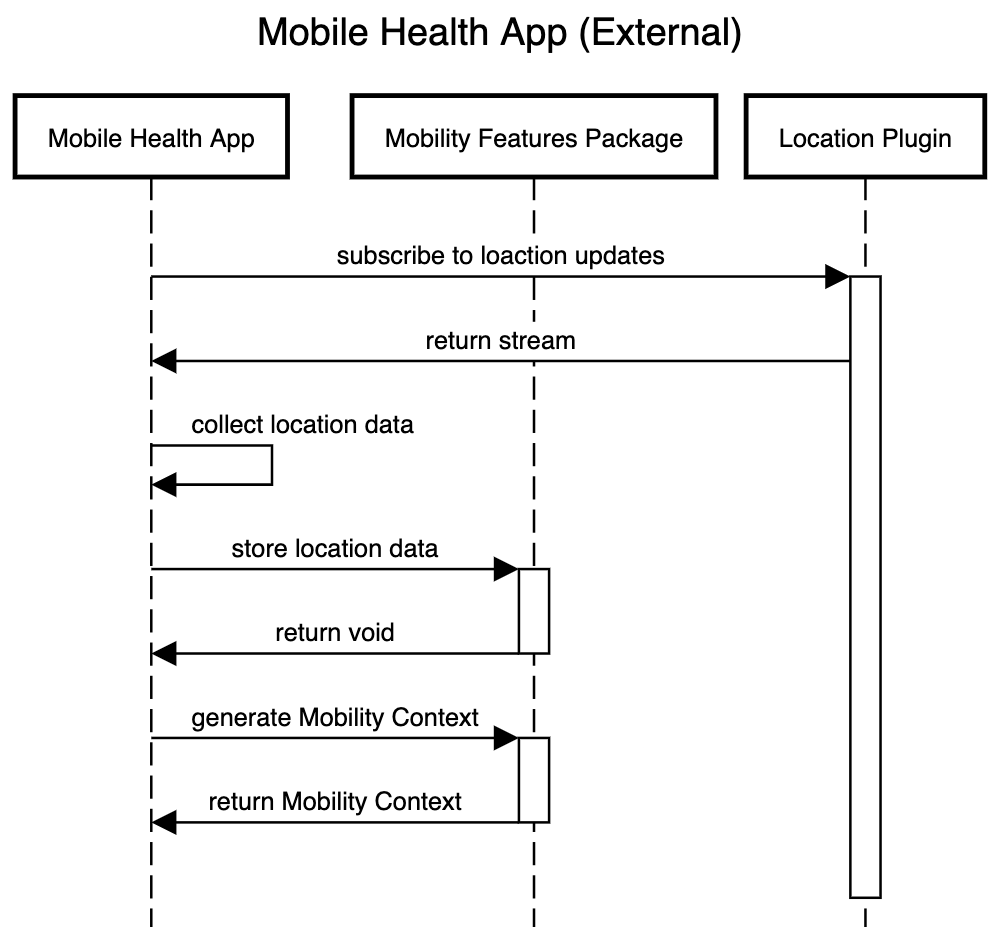
\includegraphics[width=0.8\textwidth]{images/diagrams/sequence-external.png}
\caption{Component diagram for the Mobility Feature Package from an internal point of view}
\label{fig:sequence-diagram-internal}
\end{figure}

From an internal point of view, the Context Generator component calls the Mobility Serializer for storing and loading historical data, uses the loaded data to generate a MobilityContext.

\begin{figure}[h]
\centering
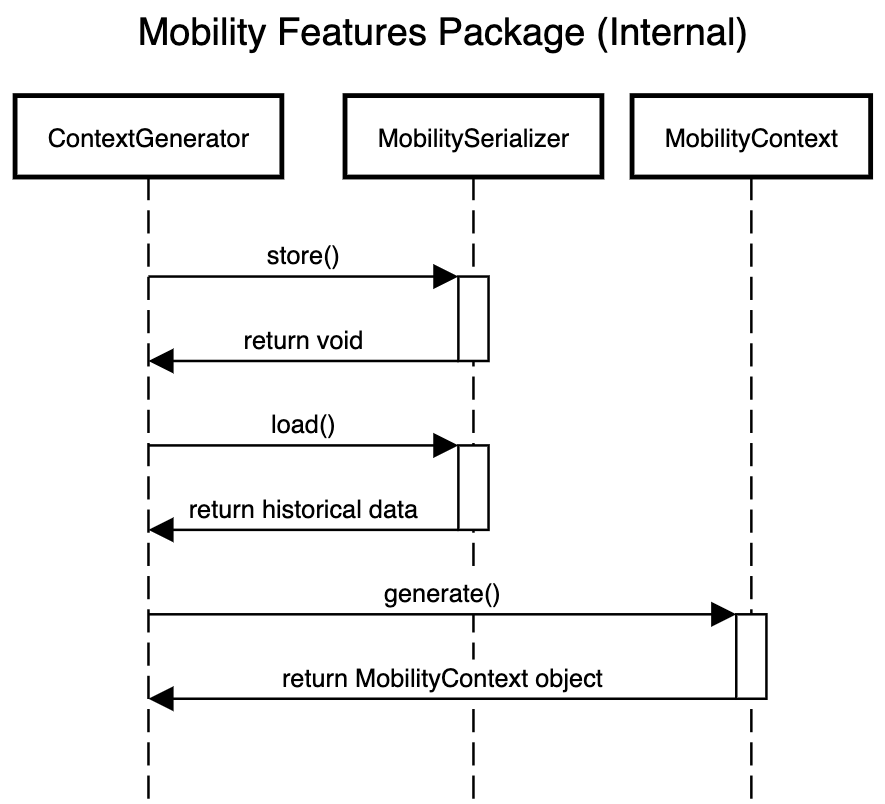
\includegraphics[width=0.8\textwidth]{images/diagrams/sequence-internal.png}
\caption{Sequence diagram for mobile health application using the Mobility Features Package, i.e. viewed externally from the package}
\label{fig:sequence-diagram-external}
\end{figure}